\chapter{Introduction and Motivation}
\label{text:introduction}
Autonomous systems play an increasingly fundamental role in our society. A study of McKinsey in 2017 showed the large effects increasing automatic will have on the economy; one of the key inside of the study is that even as automation causes declines in some occupations, it will change many more, with estimated 60 percent of occupations of which at least 30 percent of constituent work activities will be automated \footnote{\href{https://www.mckinsey.com/~/media/McKinsey/Featured\%20Insights/Future\%20of\%20Organizations/What\%20the\%20future\%20of\%20work\%20will\%20mean\%20for\%20jobs\%20skills\%20and\%20wages/MGI-Jobs-Lost-Jobs-Gained-Report-December-6-2017.ashx}{Jobs lost, Jobs gained: Workforce transitions in a time of automation - McKinsey Global International}}. The International Federation of Robotics, an association of unilateral robotics societies and companies operating in the field, illustrated the rise of service robots in many fields, such as logistics, healthcare or agriculture, in its annual report 2019.\footnote{\href{https://ifr.org/downloads/press2018/IFR\%20World\%20Robotics\%20Presentation\%20-\%2018\%20Sept\%202019.pdf}{Annual Report 2019 - IFR}} Next to the field of fully autonomous robots there also they state an increasing share of collaborative robots, e.g. assisting object retrieval in warehouses or cleaning in hospitals.

\begin{figure}[!ht]
\begin{center}
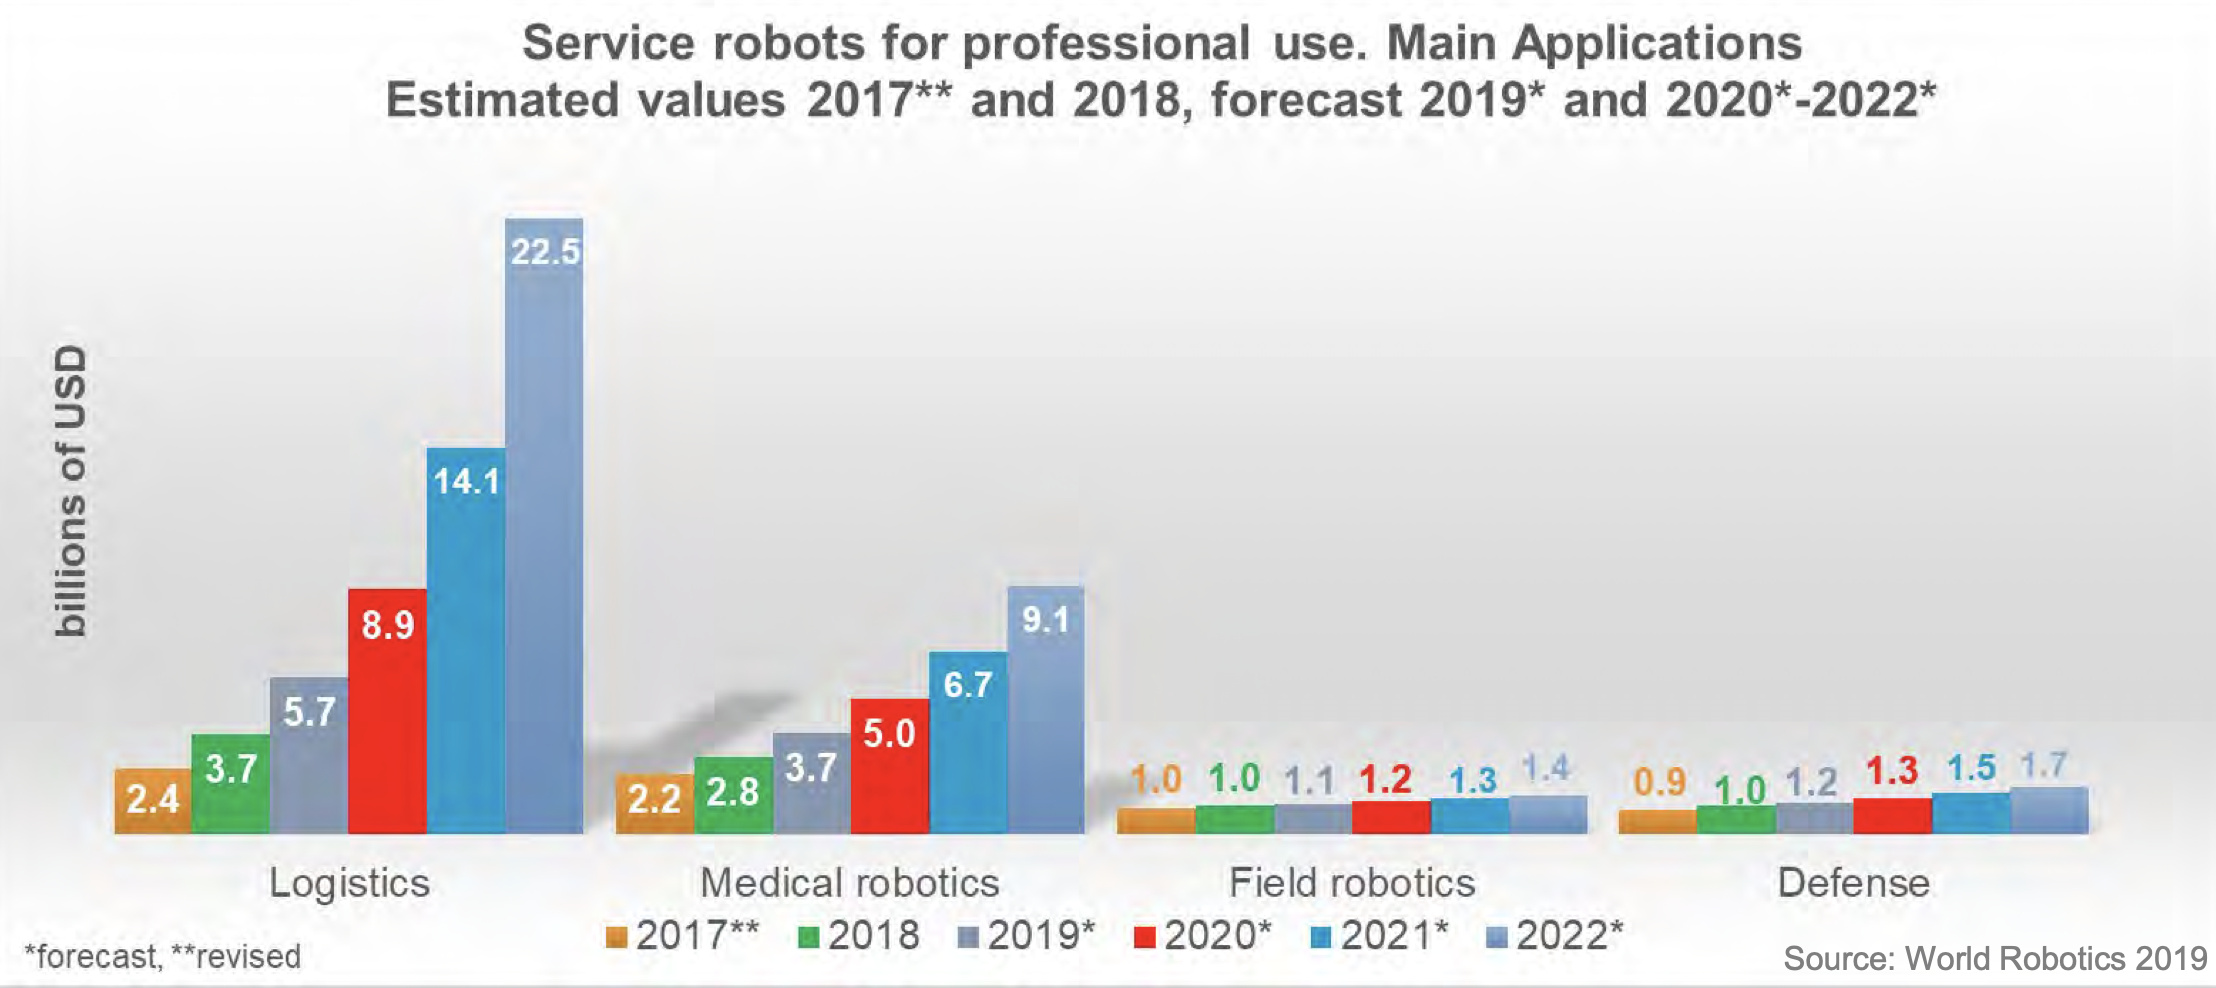
\includegraphics[width=\imgwidth]{images/service_robotics.png}
\captionof{figure}{Estimated global revenue of service robots by professional use from 2017 until 2020}
\label{img:service_robotics}
\end{center}
\end{figure}

A blog article published by the Management Review of MITs Sloan School stated that this development might be vastly accelerated due to the societal effects of COVID-19.\footnote{\href{https://sloanreview.mit.edu/article/ai-robots-and-ethics-in-the-age-of-covid-19/}{AI, Robots, and Ethics in the Age of COVID-19 - MIT Sloan Management Review}} A perfect example of this development can be observed in the Bishan-Ang Mo Kio park in Singapore, where the robot dog "Spot" is patrolling to monitor social distancing measures. While in the example the robot still is piloted by a human controller, in future these systems should work fully autonomously.\footnote{\href{http://www.straitstimes.com/singapore/meet-spot-the-safe-distancing-robot-on-trial-in-bishan-amk-park}{Meet Spot, the safe distancing robot on trial in Bishan-AMK Park - The Straits Times}}

\begin{figure}[!ht]
\begin{center}
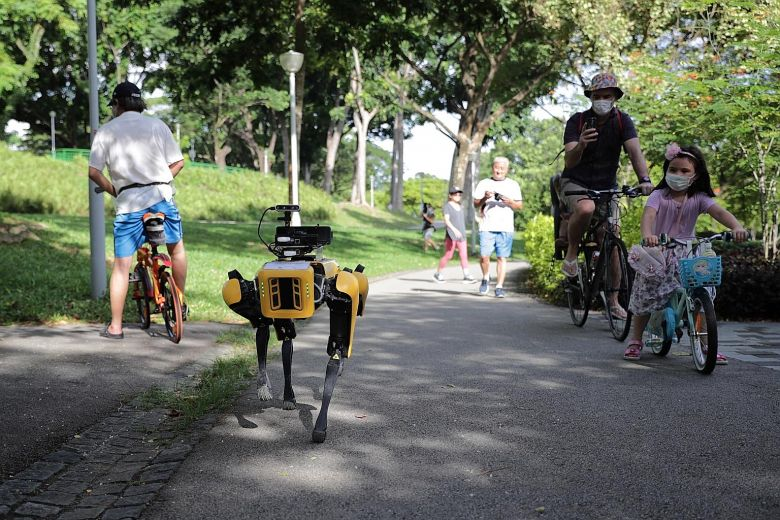
\includegraphics[width=\imgwidth]{images/spot.jpg}
\captionof{figure}{Boston Dynamics robot dog Spot patrolling in Bishan-Ang Mo Kio Park in Singapore in May 2020}
\label{img:spot_in_park}
\end{center}
\end{figure}

Summarising, robots taking part in a growing part of our social and economical life, however, an efficient but more importantly safe interaction between robots and humans is crucial for its success, interactions such as walking in between them as in the example displaying in Figure \ref{img:spot_in_park}.
\newline
In interactive multi-agent scenarios the standard control loop of percepting the sensor input, predicting, planning and executing the action \cite{Siegwart2011} is extended by a backward loop, due to the effects of the planned actions which have to be taken into account. Therefore after planning some future trajectory of the robot, a simulation predicts the behaviour of the interacting agents, conditioned on the planned robot trajectory (comp. Figure \ref{fig:control_loop_interactive}, idea from \cite{Romanski2019}). In order to guarantee interaction properties such safety usually the planner has to take into account the behaviour of the other agents. However, as the term interactive implies, this behaviour depends on the planned robot trajectory. This intrinsic dependence loop makes it especially hard to deal with interactive scenario. 

\begin{figure}
\begin{center}
\tikzstyle{block} = [draw, rectangle, minimum height=3em, minimum width=6em]
\tikzstyle{sim} = [draw, fill=cyan, rectangle, minimum height=3em, minimum width=6em]
\tikzstyle{input} = [draw, fill=orange, rectangle, minimum height=3em, minimum width=6em]
\tikzstyle{output} = [draw, fill=yellow, rectangle, minimum height=3em, minimum width=6em]
\begin{tikzpicture}[align=center, node distance=3cm,>=latex']

    \node[input, name=input](input){Sensor Input};
	\node [block, right of=input] (perception){Perception};
    \draw [->] (input) -- node {} (perception);
	\node [block, right of=perception] (prediction){Prediction};
	\draw [->] (perception) -- node[name=x] {} (prediction);
	\node [block, right of=prediction] (planning){Planning};
    \draw [->] (prediction) -- node[name=y] {} (planning);
	\node [sim, below of=y] (simulation){Simulation};
	\node [output, right of=planning] (actors){Actors};
	\draw [->] (planning) -- node[name=z] {} (actors);
	\draw [->] (z) |- (simulation);
	\draw [->] (simulation) -| (x);

\end{tikzpicture}
\captionof{figure}{Robotics control loop for interactive multi-agent scenarios}
\label{fig:control_loop_interactive}
\end{center}
\end{figure}

Within the field of safe navigation in crowded areas, especially in for human crowds. While humans use their "theory of mind", for reasoning about the other human's actions \cite{Gweon2013}, robots do not have this capacity (so far). As a consequence approaches that act in this highly dynamic, uncertain and multi-modal environment try to reduce the complexity of the problem by making strong assumptions about the human behaviour and/or by avoiding any risk. These approaches lack at least one of these properties, that are crucial for working reliable and safe near humans: 

\begin{itemize}
\item Realistic representation of the real, complex human behaviour including its multi-modal, probabilistic and highly dynamic nature
\item Certifiability by being able to explain and predict the outcome (or at least bounding it) in order to guarantee safety 
\item Computational efficient for real-time application
\end{itemize}

\section{Goals}
\label{text:introduction/goals}
In this work I want to tackle safe navigation in human crowds by combining two of the main paradigms in this field, trajectory optimisation algorithms and deep learning prediction models. I want to come up with an algorithm that both takes the complex human behaviour into account, without the need of strong assumptions about human behaviour, while still being able to track and guarantee properties of the resulting robot trajectory. Also I want to re-frame the problem of safe navigation from pure travel-time or safety optimally to an interaction-aware objective, minimising the disturbance the robot causes on the human behaviour, e.g. to not disrupt doctors in an hospital floor or the pedestrians strolling in the park mentioned above, while guaranteeing safety and reaching the goal when possible.
\newline
Therefore I will use a state-of-the-art deep learned probabilistic and multi-modal pedestrian trajectory prediction model combined with a shooting trajectory optimisation algorithm. To inform the gradients of its objective function, I will not use the model's output but the prediction models internal structure itself in order to optimally exploit the "hidden" information about the interactions with other pedestrians and the robot that are stored in the latent representations of the deep learned model. Thereby the main objective of the algorithm is not to reach the goal in the smallest possible robot travel-time, but to disturb the surrounding humans as less as feasible while still reaching the robot's goal. Additionally, a Hamilton-Jacobi reachability based constraint will be used for guaranteeing a safe interaction.  

\section{Outline of Work}
\label{text:introduction/outline}
This thesis contains five parts. Chapter \ref{text:introduction} motivates this work and provides insights into the challenges as well as possible applications, defines its goals and gives a brief overview of the solution developed within the thesis. Chapter \ref{text:related_work} introduces the reader into related work in the areas of pedestrian prediction model, controls \& decision making algorithms focussing on interaction between robots and humans, types of trajectory optimisation algorithms and to technical notions of safety. Chapter \ref{text:approach} deep dives into the algorithm developed within this work, starting with a more detailed summary and continuing with a detailed description and explanation of every of its parts. Chapter \ref{text:experiments} validates the approach by presenting experimental results for different settings and scenarios, measuring its performance on baselines and discussing the results. Finally, chapter \ref{text:conclusion} concludes the work and gives an outlook for future research directions.

\section{Statement of Contributions}
\label{text:introduction/contributions}

%todo: statement of contributions
